
% Define listing style for yaml
\newcommand\YAMLcolonstyle{\color{black}\bfseries\small}
\newcommand\YAMLkeystyle{\color{black}\mdseries\small}
\newcommand\YAMLvaluestyle{\color{green}\mdseries\small}

\makeatletter

% here is a macro expanding to the name of the language
% (handy if you decide to change it further down the road)
\newcommand\language@yaml{yaml}

\expandafter\expandafter\expandafter\lstdefinelanguage
\expandafter{\language@yaml}
{
  keywords={true,false,null,y,n},
  keywordstyle=\color{darkgray}\bfseries,
  basicstyle=\YAMLkeystyle,                                 % assuming a key comes first
  sensitive=false,
  comment=[l]{\#},
  morecomment=[s]{/*}{*/},
  commentstyle=\color{purple}\ttfamily,
  stringstyle=\YAMLvaluestyle\ttfamily,
  moredelim=[l][\color{orange}]{\&},
  moredelim=[l][\color{magenta}]{*},
  moredelim=**[il][\YAMLcolonstyle{:}\YAMLvaluestyle]{:},   % switch to value style at :
  morestring=[b]',
  morestring=[b]",
  literate =    {---}{{\ProcessThreeDashes}}3
                {>}{{\textcolor{red}\textgreater}}1     
                {|}{{\textcolor{red}\textbar}}1 
                {\ -\ }{{\mdseries\ -\ }}3,
}

% switch to key style at EOL
\lst@AddToHook{EveryLine}{\ifx\lst@language\language@yaml\YAMLkeystyle\fi}
\makeatother

\newcommand\ProcessThreeDashes{\llap{\color{cyan}\mdseries-{-}-}}


\definecolor{codegreen}{rgb}{0,0.6,0}
\definecolor{codegray}{rgb}{0.5,0.5,0.5}
\definecolor{codepurple}{rgb}{0.58,0,0.82}
\definecolor{backcolour}{rgb}{0.95,0.95,0.92}

\lstdefinestyle{mystyle}{
    backgroundcolor=\color{backcolour},   
    commentstyle=\color{codegreen},
    keywordstyle=\color{magenta},
    numberstyle=\tiny\color{codegray},
    stringstyle=\color{codepurple},
    basicstyle=\ttfamily\footnotesize,
    breakatwhitespace=false,         
    breaklines=true,                 
    captionpos=b,                    
    keepspaces=true,                 
    numbers=left,                    
    numbersep=5pt,                  
    showspaces=false,                
    showstringspaces=false,
    showtabs=false,                  
    tabsize=2,
    xleftmargin=15pt
}

\lstset{style=mystyle}

\chapter{Implementation} \label{chp:Implementation}
In this chapter we will take a look at different parts of the implementation. We will begin by discussing some general implementation notes in Chapter \ref{sec:ImplementationNotes} and the continue to present our experimentation environment called \textit{baselines lab} in Section \ref{sec:BaselinesLab}. We then talk about the particle simulation environment, including different scenarios from the original implementation of Huang et al. in Section \ref{sec:MazeEnvironment}.

\section{General Implementation Notes} \label{sec:ImplementationNotes}
Before talking about the actual implementation we want to talk a little bit about our general design choices. As a programming language we chose to use Python 3 \cite{van2011python, pythonWebsite}. Python is an interpreted high-level programming language with itself is written in C. Even though it is interpreted and thus may be slower than languages like C or C++, the easy integration of high-performance libraries which also scale into distributed systems make applications developed in python very fast. In the past years almost every ML library is developed for python making Python an ideal choice for data-science and machine learning projects.

The popularity of machine learning has lead to the developed of a number of libraries which support the creation and training of artificial neural networks. Modern libraries also especially leverage the computing power of the GPU to accelerate the computation of large matrix operations. Many of the libraries support more or less the same functionality, but may have a very different style of how certain things can be achieved. Currently the two most popular libraries for machine learning are PyTorch \cite{paszke2019pytorch} and Tensorflow \cite{abadi2016tensorflow}, we decided to use the latter. This decision was made in conjunction with our second big backend library which extends Tensorflow for reinforcement learning: Stable-Baselines \cite{stable-baselines}. Stable baselines offers high-quality implementations of many RL algorithms which are partially forked from the OpenAI Baselines project \cite{baselines}. While Google offers their own reinforcement library under the name TF-Agents \cite{TFAgents} we found that it currently is in a too early development state and thus not stable enough for the course of this thesis.

Since Python offers the easy integration of additional libraries we also make use of a number of additional libraries, most notably:
\begin{itemize}
    \item OpenAI Gym \cite{openAIgym} for a standardized environment creation as well as the integration of the Atari environments for testing purposes.
    \item OpenCV \cite{opencv_library} for image preprocessing.
    \item Numpy \cite{oliphant2006guide} for fast matrix computations.
    \item Optuna \cite{akiba2019optuna} for automated hyperparameter search.
\end{itemize}

\section{Baselines Lab} \label{sec:BaselinesLab}
To test out various combinations of reinforcement learning algorithms, their settings with different environments and environment settings we need a flexible and easy configurable program which also gives us the possibility to monitor the performance and create evaluations of trained models. While there already exist some projects which offer some of these features we did not find a project which was fully suited for our needs. The stable-baselines co-project baselines zoo \cite{rl-zoo} had to few options for the configuration of algorithms and while other libraries like slm-lab \cite{kenggraesser2017slmlab} did fit our need for configurability, they did not offer enough reinforcement learning algorithms. Therefore we decided to build our own lab environment on top of stable-baselines which we call \textit{Baselines Lab}.

\subsection{Basic Functions} \label{sec:blFunctions}
In this section, we want to go over the basic functions of Baselines Lab. We will start with an overview of the main functions and then give a little more detail on some of the most important features. 

When starting the lab, we have to choose between one of the three different lab modes:

\begin{enumerate}
    \item The \textit{train} lab mode can be used to train a new model.
    \item The \textit{enjoy} lab mode can be used to watch a model in action and/or evaluate its performance.
    \item The \textit{search} lab mode can be used to perform an automated hyperparametersearch. We will talk more about the search mode in Section \ref{sec:blSearch}.
\end{enumerate}

When starting a session, we also need to specify a \textit{lab configuration file} which can be written in JSON or YAML. Let us take a look at the easiest form of a config file which specifies all mandatory parameters:

\begin{figure}[h]
    \lstinputlisting[language=yaml]{figures/implementation/simple_config.yml}
    \caption{Basic lab configuration file in YAML.}
\end{figure}


We can see that the basic lab configuration only requires a handful of parameters which define which RL algorithm should be used in conjunction with which neural network, which environment and for how long the model should be trained. In general there are three basic categories for the parameters defined by the three main keywords: 

\begin{enumerate}
    \item The \textit{algorithm} keyword specifies all parameters related to the used reinforcement learning algorithm. The parameters which can be set are dependent on the used algorithm and correspond directly to the parameters of the stable-baselines documentation \cite{stable-baselines-docs}. The only exception to this is the policy, which defines the used neural network. The policy type - corresponding to its registered class - is defined under the \textit{name} keyword. Additional policy arguments can be directly specified under the \textit{policy} keyword.
    \item The \textit{env} keyword specifies all parameters which are directly related to the environment. The only mandatory parameter is the name of the environment corresponding to its registered gym entry. The env keyword allows for a lot of parameters regarding observation preprocessing like frame stacking or normalization. We included a full list in Appendix TODO. 
    \item  The \textit{meta} keyword describes all meta parameters for the training process. For example we can define how often the model should be saved or evaluated, which random seed should be used or how many times the experiment should be repeated. For a full list of available arguments, see Appendix TODO.
\end{enumerate}

Independent of the used lab mode, the same configuration file can be used. However some functions may depend on certain configurations. If we want to inspect an already trained model, we must specify a log directory under "meta" when training. This will result in models being saved periodically during training at the given location. The latest or best models can then be inspected in enjoy mode by just starting the lab with the same configuration file. 

\paragraph{Automated Saving and Loading.}
We already mentioned that it is possible to automatically save and load models, but we want to describe the procedure a little bit more in depth. The first question is what needs to be serialized when training the model. The answer to this depends on the used configuration, since it may include components which need to be saved additionally to the parameters of neural network. For example parameters if we normalized the observations of the environment using a running mean, we need to save that running mean, otherwise our model would not be able to perform after loading it. A single checkpoint therefore may contain multiple files depending on the current configuration.

If a log directory location is specified the lab will create a log directory with a current timestamp. Models (and additional components) will be periodically saved during training to a subdirectory called \textit{checkpoints}. On default, the lab keeps the last 5 checkpoints and the model which had the best performance during training. This behavior can also be changed (see Appendix TODO).

The checkpoints created during training can be used in enjoy mode or if we want to continue training in the future. To continue training, we just add a \texttt{trained\_agent} keyword to the algorithm configuration and specify weather we want to load the \textit{last} or the \textit{best} checkpoint. In enjoy mode the best checkpoint is selected on default. To change this behavior we can specify a \texttt{-{}-type} command line argument and set it to \textit{last}.

\paragraph{Automated Evaluation}
Models are automatically evaluated during training. This evaluation is done periodically to determine the current model performance. Evaluation can be done in three different modes depending on the desired tradeoff between evaluation accuracy and speed:

\begin{enumerate}
    \item \textbf{Fast.} Fast evaluation is not really doing a dedicated evaluation run. Instead the current results are computed by looking at the average reward and episode length over the last 100 training episodes. This procedure is very fast because the results are already computed during training, but may be inaccurate and also only represents the training behavior which might be substantially different depending on the used RL algorithm (e.g. for DQN).
    \item \textbf{Normal.} Normal evaluation uses a dedicated vectorized evaluation environment with 32 parallel instances. Because each instance is reset independently this evaluation type still might produce a small bias towards short episodes, which slightly improves results if short episodes are good and slightly worsens results if short episodes are bad. Nevertheless we found that the results do not deviate to much from the performance when executing the same model on a single environment and thus the results can be used to compare different models.
    \item \textbf{Slow.} Slow evaluation uses a dedicated evaluation environment with a single instance. This might take a lot of time during training, but produces very accurate results. 
\end{enumerate}

Evaluation can also be done outside of the train lab mode, by specifying the \texttt{-{}-evaluate} command line argument for the enjoy lab mode. The argument expects a number of episodes to test and uses the normal evaluation mode on default. If we are interested in completely accurate results we can additionally specify the \texttt{-{}-strict} option. Evaluation in enjoy mode automatically saves the evaluation results to the training log directory. 

\paragraph{Monitoring}
Monitoring the training process is very important in all machine learning areas. By logging all kinds of values we are able to determine errors in the implementation, select good hyperparameters and overall control the quality of the training process. Luckily, Tensorflow comes with an integrated monitoring system called Tensorboard which allows us to inspect the neural network and log values during training. These values can then be plotted in real time by starting the Tensorboard application (which gets automatically installed with Tensorflow). Figure \ref{fig:TensorboardExample} shows an example of the Tensorboard visualization, which can be accessed with a web browser.

\begin{figure}[ht]
    
    \begin{center}
        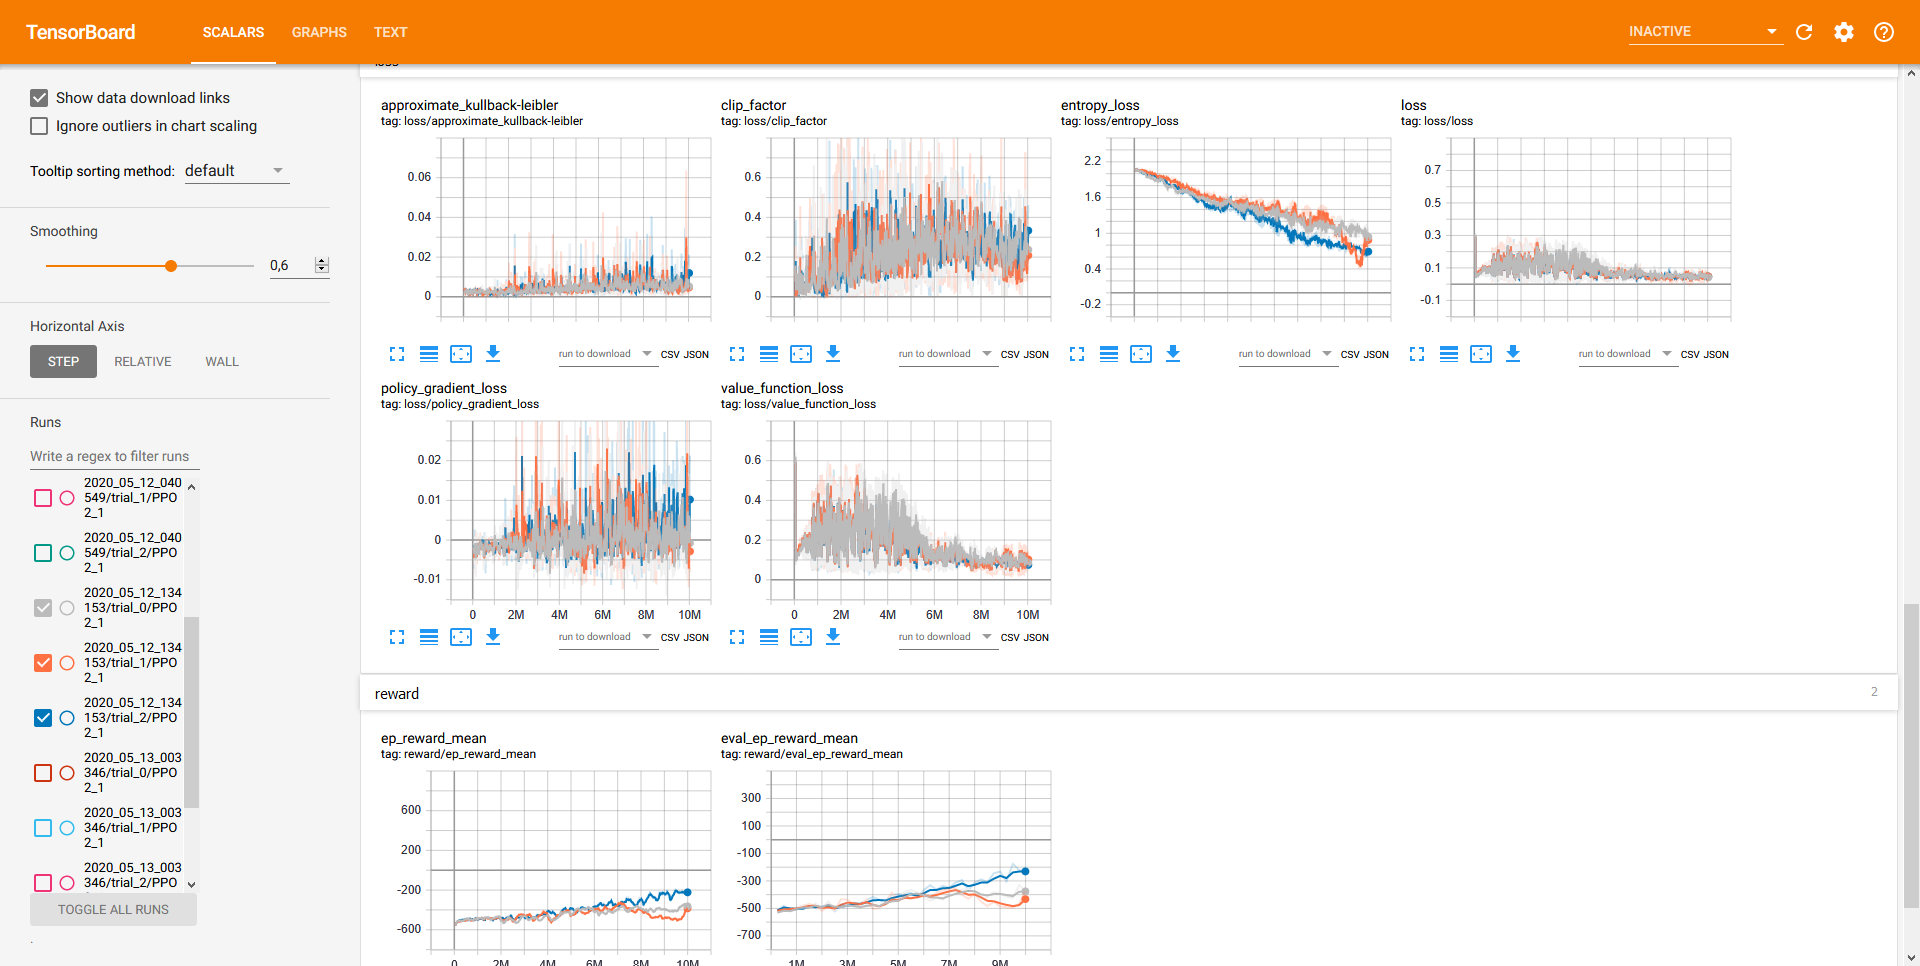
\includegraphics[clip, width=0.95\columnwidth]{figures/implementation/Tensorboard.png}
    \end{center}
    
    %\vspace*{-6pt}
    \caption[Tensorboard Example]{Example for a Tensorboard visualization.}
    \label{fig:TensorboardExample}
    %\vspace*{-12pt}
  \end{figure}

Stable Baselines already integrates Tensorboard for extended logging and visualization. Dependent on the chosen RL algorithm, Stable Baselines will log internal values like the average action advantage or the discounted reward. With Baselines Lab we extend these logging capabilities and now also include episode length and average episode reward for both training and evaluation. We also included a metric for steps per second which helps to monitor execution performance. For special modules like RND (see Section \ref{sec:blRND}) we also include module specific plots like intrinsic reward. The lab configuration is also included in the Tensorboard log file.

Tensorboard logs are created automatically at the given log directory location if the \texttt{tensorboard\_log} parameter of the algorithm is set to true.


\subsection{Random Network Distillation Module} \label{sec:blRND}
Unique RND implementation -> Staged as extension for SB3

\subsection{Automated Hyperparametersearch} \label{sec:blSearch}
Optuna and its basic functions, how to configure hyperparametersearch.

\subsection{Additional Functions} \label{sec:blAdvanced}
Automated Plots
Automated video creation (enjoy, obs).
Learning rate schedules.
Email notification


\section{The Particle Maze Environment} \label{sec:MazeEnvironment}

\subsection{Basic Implementation} \label{sec:MazeImplementation}
Reimplementation of Huangs environment. Observations, etc

\subsection{Reward Shaping} \label{sec:MazeReward}
Rewards

\subsection{Extended Models} \label{sec:ExtendedMaze}
fuzzy, physical 

\subsection{Random Instance Generation} \label{sec:RandomInstanceGeneration}
random map generation

\section{Integration of Algorithmic Approaches} \label{sec:AlgorithmIntegration}
integration


